\documentclass{slides}
\usepackage{geometry,color}
\usepackage{graphicx} % Required for inserting images
\usepackage[font=small,labelfont=bf]{caption} % Required for specifying captions to tables and figures
\usepackage{amsmath}
\usepackage{amssymb}
% \usepackage{cite}
\usepackage{algorithm}
\usepackage{algpseudocode}
% \usepackage{biblatex}
\usepackage{float}
% \usepackage{hyperref}
\geometry{screen}
\paperwidth 11.0truein
\paperheight 8.5truein
\oddsidemargin -0.25truein
\evensidemargin -0.25truein
\textheight 7in
\textwidth 9.5in
\topmargin -.8in

\newcommand{\R}{\mathcal{R}}
\newcommand{\PA}{\mathcal{P}}
\newcommand{\U}{\mathcal{U}}

%\usepackage{makeidx,multicol,cite,verbatim}
%\usepackage{amsmath,amssymb,amscd,fixmath,upgreek,amsthm,textcomp}
%\usepackage[mathscr]{eucal}% \makeindex
%\usepackage{Mngr-sli}
%\usepackage{Mngr-macros-sli}
%\raggedbottom
%%%%%%%%%%%%%%%%%%%%%%%%%%%%%%%%%%%%%%%%%%
\definecolor{dmagenta}{rgb}{.4,.1,.5}
\definecolor{007}{rgb}{.0,.0,.7}
\definecolor{dred}{rgb}{.5,.0,.0}
\definecolor{dgreen}{rgb}{.0,.5,.0}
\definecolor{dblue}{rgb}{.0,.0,.5}

\definecolor{550}{rgb}{.5,.5,.0}
\definecolor{505}{rgb}{.5,.0,.5}
\definecolor{055}{rgb}{.0,.5,.5}
\definecolor{551}{rgb}{.5,.5,.1}
\definecolor{515}{rgb}{.5,.1,.5}
\definecolor{155}{rgb}{.1,.5,.5}

\definecolor{400}{rgb}{.4,.0,.0}
\definecolor{040}{rgb}{.0,.4,.0}
\definecolor{004}{rgb}{.0,.0,.4}
\definecolor{440}{rgb}{.4,.4,.0}
\definecolor{404}{rgb}{.4,.0,.4}
\definecolor{044}{rgb}{.0,.4,.4}
\definecolor{441}{rgb}{.4,.4,.1}
\definecolor{414}{rgb}{.4,.1,.4}
\definecolor{144}{rgb}{.1,.4,.4}

\definecolor{300}{rgb}{.3,.0,.0}
\definecolor{030}{rgb}{.0,.3,.0}
\definecolor{003}{rgb}{.0,.0,.3}
\definecolor{330}{rgb}{.3,.3,.0} %
\definecolor{303}{rgb}{.3,.0,.3}
\definecolor{033}{rgb}{.0,.3,.3}
\definecolor{331}{rgb}{.3,.3,.1}
\definecolor{313}{rgb}{.3,.1,.3}
\definecolor{133}{rgb}{.1,.3,.3}

\definecolor{200}{rgb}{.2,.0,.0}
\definecolor{020}{rgb}{.0,.2,.0}
\definecolor{002}{rgb}{.0,.0,.2}
\definecolor{220}{rgb}{.2,.2,.0} %
\definecolor{202}{rgb}{.2,.0,.2}
\definecolor{022}{rgb}{.0,.2,.2}
\definecolor{221}{rgb}{.2,.2,.1}
\definecolor{212}{rgb}{.2,.1,.2}
\definecolor{122}{rgb}{.1,.2,.2}

\definecolor{violet}{rgb}{.3,.0,.9}
\definecolor{orange}{cmyk}{0,.5,.1,.0}
\definecolor{dcyan}{cmyk}{.5,.0,.0,.0}
\definecolor{dyellow}{cmyk}{.0,.0,.5,.0}
\definecolor{cm}{cmyk}{1,.0,.0,.0}
\usepackage{graphicx}
\usepackage{color}

% red,blue,yellow,magenta,cyan,green,black



%%%%%%%%%%%%%%%%%%%%%%%%%%%%%%%%%%%%%%%%%%
\title{\color{007}\Large From Lagrange to Whittle and back}\author{\large Vivek Borkar\\
IIT Bombay\footnote{\large Joint work with Pratik Shah (IITB $\to$ GATECH),\\ Konstantin Avrachenkov (INRIA Sophia Antipolis)}}\date{\large GAME-ARTS\\ \ \\ Indian Institute of Science, 19th July, 2024}
%%%%%%%%%%%%%%%%%%%%%%%%%%%%%%%%%%%%%%%%%%
\begin{document}
\maketitle
%%%%%%%%%%%%%%%%%%%%%%%%%%%%%%%%%%%%%%%%%%
%%%%%%%%%%%%%%%%%%%%%%%%%%%%%%%%%%%%%%%%%%
\newpage
{\large \color{144} 
 
\textbf{PRELUDE:} Restless bandits

Consider $N$ Markov decision processes {\color{red} (`\textit{arms}')} denoted \\ by $X^i_n, n \geq 0,$ on finite or countable state spaces $S_i$, with controls $U^i_n, n \geq 0,$ in a common action space $\U = \{0,1\}$.

Each (say, $i$th) arm has two alternative modes, {\color{red} `active', i.e., $U^i_n = 1$,} and {\color{red} `passive', i.e., $U^i_n = 0$}, 

corresponding to transition probabilities for the $i$th arm 
{\color{red} $p^i(j|k,u),  j,k\in S_i,$} \\
and rewards {\color{red} $R^i(j,u), j \in S_i$}, for {\color{red} $u \in U$}.\\ (Usually, $R^i(\cdot, 1) > R^i(\cdot,0)$.)

\newpage

The arms are coupled through the constraint
{\color{red} $$\sum_{i=1}^NU^i_n = M,$$}
for some $1\leq M < N$, i.e., only $M$ arms can be active. 

Compare with classical `rested' bandits: in passive mode, the arm does not evolve. 

For rested bandits, optimal policies such as the Gittins index (Gittins, '79) are known.

}

\newpage

 {\large \color{dblue}
 
 The restless bandit  problem is PSPACE hard\\ (Papadimitriou and Tsitsiklis, '99). 
 
 Whittle introduced a heuristic that works well in practice (Whittle, '88).
 
 It can be shown to be asymptotically optimal in a certain sense (Weber and Weiss, '90).
 
 
 \newpage
 

 
 \textbf{Recap of (Whittle, '88):}
 
 Whittle considered the average reward:
 $$\lim_{n\uparrow\infty}\frac{1}{n}\sum_{m=0}^{n-1}E\left[\sum_{i=1}^NR^i(X^i_m,U^i_m)\right]$$
 He replaced the `per stage' constraint of `$M$ out of $N$' by an `average' constraint:
 $$\lim_{n\uparrow\infty}\frac{1}{n}\sum_{m=0}^{n-1}E\left[\sum_{i=1}^NU^i_m\right] = M.$$
This is a constrained MDP that can be reduced to an unconstrained MDP by using the Lagrange multiplier $\lambda^*$

\newpage

The new problem is:  Maximize
$$\lim_{n\uparrow\infty}\frac{1}{n}\sum_{m=0}^{n-1}E\left[\sum_{i=1}^NR^i(X^i_m,U^i_m) + \lambda^*(\sum_{i=1}^NU^i_m-1)\right],$$
where $\lambda^* :=$ the Lagrange multiplier. 

Whittle used this to motivate a {\color{red} `subsidy for passivity'} given by $\lambda$, i.e., the reward for remaining passive is now $R^i(x,0) + \lambda$.

He defined {\color{red} (Whittle) indexability} as the property that for each arm,  the set of states for which it is optimal to remain passive {\color{red} increases} from the empty set to the entire state space as $\lambda$ is increased from $-\infty$ to $+\infty$.

\newpage

For problems that are (Whittle) indexable, he defined the {\color{red} (Whittle) index} for state $k$ as the value $\lambda(k)$ of the subsidy for which both active and passive modes become equally desirable at state $i$.

The {\color{red} (Whittle) index policy} then is to rank order $\lambda(X^i_n)$'s in decreasing order at each time instant $n$, and render the top $M$ arms active, breaking ties if any according to some pre-specified protocol.

\newpage

Recall the dynamic programming equation for average reward with subsidy : for $1 \leq i \leq N, k \in S_i$, 
$$V^i(k) = \max_{u\in\{0,1\}}\Big(R^i(k,u) + \lambda I\{u=0\} - \beta^i + \sum_jp(j|k,u)V^i(j)\Big),$$
where $\beta_i :=$ the optimal reward.

Define the `Q-value' as the expression :
$$Q_\lambda^i(k,u) := R^i(k,u)  - \beta^i + \sum_jp(j|k,u)V^i(j).$$
Then $\lambda(k)$ satisfies
$$ \lambda(k) = Q_{\lambda(k)}^i(k,1) - Q_{\lambda(k)}^i(k,0).$$

\newpage

Q-values satisfy their own dynamic programming\\ equation:
\begin{eqnarray*}
Q_\lambda^i(k,u) &=& R^i(k,u) + \lambda I\{u=0\} - \beta^i + \\
&& \sum_jp(j|k,u)\max_{u'\in\{0,1\}}Q_\lambda^i(j,u').
\end{eqnarray*}
This can be solved by relative value iteration, policy\\ iteration, linear programming, etc.

But it needs to be solved for {\color{red} each state $k$}, which is in particular very tedious in the heterogeneous case\\ (i.e., when the MDPs are not identical).

\newpage

In a few lucky situations, explicit expressions are\\ available:

Ansell, Glazebrook, Nino-Mora, O'Keeffe '02 

Rahunathan, B., Cao, Kumar '08

Liu, Zhao '10;  \ \ 
Avrachenkov, B. '16 

Yu, Xu, Tong '18; \ \ 
Tripathi, Modiano '19  

Sombabu, Mate, Moharir, Manjunath '22
}

\newpage
{\large \color{dred} 

\textbf{The Lagrange index:}

Recall the Lagrangian formulation. The {Lagrange index} can be defined as
$$\Lambda (k) := Q_{\lambda^*}(k,1) - Q_{\lambda^*}(k,0).$$
The Lagrange index policy is to rank order at time $n$ the $\Lambda(X^i_n), 1 \leq i \leq N,$ in decreasing order and render the top $M$ active, breaking ties if any appropriately.

\newpage

\textbf{Advantages:}

In case an explicit expression for the Whittle index is not available, the Lagrange index needs much less computation because we work with a fixed $\lambda^*$.  

Also, it does not require Whittle indexability.

Prior work for finite horizon problems:

Brown, D. B., and Smith, J. E. (2020).
Index policies and performance bounds for dynamic selection problems.
Management Science, 66(7), 3029-3050.

\newpage

An alternative family of indices based on the {\color{red} Linear\\ Programming (LP) } formulation of MDPs, dubbed `LP-priority policies'  has been introduced in (Verloop, '16). 

See also (Xiong, Li, Singh '22) for related work. 

Of these, the `LP-index policy' flagged by (Gast, Gaujal,  Yan '23) is essentially identical to the Lagrange policy, in that it uses $Q(i,1) - Q(i,0)$ values to compare the arms. 

\newpage

Our experiments show comparable performance of the Lagrange index policy to the Whittle index policy on Whittle indexable problems, and better performance on problems that are not Whittle indexable.

The new proof of asymptotic optimality  under the `global attractor condition' introduced in (Verloop '16), (Gast, Gaujal and Yan, '23) is given using exchangeability and de Finetti's theorem.

\newpage

The new proof proceeds in following steps:

1.\ In the $N \to \infty$ limit, the arms form an exchangeable sequence (i.e., the joint distributions are invariant under permutations). By de Finetti's theorem, they are independent conditioned on the $\sigma$-field of exchangeable events ($:=$  events invariant under permutations).

2.\ The limiting process prescribes how the active mode is assigned to the arms with the top values of the Lagrange index. 

3.\ The `global attractor principle' imposes certain `deterministic' constraints on this allotment. 

4.\ It can be argued that for conditional independence to be compatible with this, each arm must be separately, optimally controlled. 

This uses a characterization of optimal stationary policies for constrained MDPs due to (Beutler and Ross, '85), which says that for a single constraint, one needs to randomize at most between two actions at a single state.



\newpage

{\large \color{144}

\begin{center}
\textbf{\Large Numerical experiments}
\end{center}
\newpage
\textbf{Calculating Lagrange indices using tabular Q-Learning}
\begin{algorithm}[H]
\begin{small}
\begin{algorithmic}[1]
    \State Initialize $\lambda^*$, Q(s,a) for all states and actions, $\epsilon$=0.1.


    % \Function{VisualizationRecommendation}{$B$, $D$, $M$}:
    % \State $\epsilon \gets \text{initialize an error value for terminate condition}$
    % \State $S \gets [S_1, S_2, S_3, ...., S_{
    % |S|}]$  $\text{($|S_{k+1}| > |S_{k}|$ $\forall k \in [1, |S| - 1]$)}$
    % \State $m$ $\gets$ $\text{number of columns of $S_k$}$
    % \State $n$ $\gets$ $\text{number of features per column}$
    \For {n\;=\;1:\;$n_{end}$}
        \State Update $\alpha(x)$ and $\beta(n)$ as:
        $\alpha(x)=\frac{1}{\lceil{x\backslash5000}\rceil+1}$ $\beta(n)=\frac{1}{\lceil{nlog(n)\backslash5000}\rceil+1}$
        \State Choose action $a_{n}^i$ for each arm i in an $\epsilon$-greedy fashion
        \State Update $s_{n+1}^i$ and reward $r_n^i$ from $s_{n}^i$ and $a_{n}^i$ for every arm i
        
        \State Update ($s_n^i$,$a_n^i$) Q-values for each arm i as:
        \Statex\begin{small}$Q_{n+1}(s_n,a_n)\gets(1-\alpha(\nu(n,s_n,a_n)))Q_n(s_n,a_n)+\alpha(\nu(n,s_n,a_n))((1-a_n)(r_o(s_n)+\lambda_n^*)+a_nr_1(s_n)+\underset{v\epsilon\{0,1\}}{max}Q_n(s_{n+1},v)-\frac{1}{2d}\sum\limits_{k\in S}Q_n(k,0)+Q_n(k,1))$\end{small}
        \State Update common subsidy for passivity for all arms $\lambda^*$ as: $\lambda_{n+1}^*=\lambda_n^*+\beta(n)(\sum\limits_{i=1}^{i=N}a_n^i-M)$
        
        % \State Decrement $\epsilon$ as $\epsilon_{n+1}=max(0.01,\epsilon_{n}*0.99)$
        % \State $total \textunderscore cost \gets 0$
        % \State $\Tilde{y_{k}} \gets$ \text{ranking score of the viz produced using all the features predicted by P}
        % \State $terminate \textunderscore flag \gets False$
        % \While{not $terminate \textunderscore flag$}
        %     \If{$random$ in $[0,1) \leq Pr_{\text {rand}}$} 
        %         \State $ij \gets$ \text{index of a randomly selected unknown feature}
        %     \Else
        %         \State $ij$ $\gets$ $Q(x^{k, t})$ $\text{(index of the feature with the maximum Q value)}$
        %     \EndIf
        %     \State $x^{k, t+1} \gets \text{acquire $f_{ij}$ and unmask it}$
        %     \State $P(x^{k, t}) \gets \text{ranking score predicted using the feature set $x^{k, t}$}$
        %     \State $total \textunderscore cost \gets total \textunderscore cost +\boldsymbol{c}_{\boldsymbol{ij}}$ 
        %     \State $r_{ij}^{k, t} \leftarrow \frac{\left\|\operatorname{P}\left(\boldsymbol{x}^{k,t}\right)-\operatorname{P}\left(\boldsymbol{x}^{k, t+1}\right)\right\|}{\boldsymbol{c}_{ij}} $
        %     \State \text{push} $\left(\boldsymbol{x^{k, t}}, \boldsymbol{x^{k, t+1}}, ij, r_{ij}^{k, t}, \tilde{y_k}\right)$ \text{into the replay memory}
        %     \State $t \leftarrow t+1$
        %     \If{$total \textunderscore cost \geq B$}
        %         \State $terminate \textunderscore flag \gets True$
        %         \State $\hat{y_k} \gets P(x^{k, t})   \text{predicted viz ranking  score on subset of features $x^{k, t}$}$
        %     \EndIf
        %     \State \text{loss} $\gets$ $L(\Tilde{y_k}$,$\hat{y_k})$
        %     \If{$update \textunderscore condition$}
        %         \State \text{train \textunderscore batch} $\gets$ \text{random mini-batch from the replay memory}
        %         \State \text{update Q and target Q networks using train batch }
        %     \EndIf
                
        % \EndWhile
        % \If{$\epsilon > loss$}
        %     terminate loop
        % \EndIf
    \EndFor
    \State Calculate the new index for each arm i where the current state of arm is represented by k:
        \Statex\hspace*{5mm} $\delta(k)=Q_{\lambda^*}(k,1)-Q_{\lambda^*}(k,0)$
\end{algorithmic}
\end{small}
\end{algorithm}

\newpage
We present 4 approaches for finding the LP indices:
\begin{itemize}
    \vspace{-15mm}
    \item \textbf{A}. Using a single Q-value matrix shared across all homogenous arms of the same type
    \vspace{-15mm}
    \item \textbf{B}. Using a different Q-value matrix for each arm, and hence the updates change the Q-values of the corresponding arm only
    \vspace{-15mm}
    \item \textbf{C}. Allowing a maximum budget number of arms only to be pulled even during the training phase. 
    \vspace{-15mm}
    \item \textbf{D}. Single arm analysis
    % Suppose there are total N arms out of which M arms is the budget. Let there be K different types of arms with $l_K$ arms belonging to each type such that
    % $\sum\limits_{j=1}^{j=K}{l_j}=N$. 
    % \\ The update for the common subsidy is
    % $\lambda_{n+1}^*=\lambda_n^*+\beta(n)(\sum\limits_{t=i}^{t=n}(\sum\limits_{i=1}^{i=N}(\sum\limits_{j=1}^{j=K}{l_j}*a_t^i*I\{i \in j\}/N))/n-M/N)$
    % Where $I\{i \in j\}$ indicates if arm i belongs to the $j^{th}$ class
\end{itemize}
\newpage
\textbf{Restart Bandits}\\
We consider a “restart problem” with state space $S = \{0, 1, 2, 3, 4\}$, where in the passive mode (u = 0) an arm has tendency to go up the state space whereas in the active mode (u = 1) the arm restarts from state
1 with probability 1, i.e.,
\begin{align*}
P_0=
\begin{bmatrix}
0.1 & 0.9 & 0&0&0\\
0.1 & 0 & 0.9 & 0 &0\\
0.1&0&0&0.9&0\\
0.1&0&0&0&0.9\\
0.1&0&0&0&0.9
\end{bmatrix}
\hspace{1mm} \text{and} \hspace{1mm}
P_1=
\begin{bmatrix}
1 & 0 & 0&0&0\\
1 & 0 & 0 & 0 &0\\
1&0&0&0&0\\
1&0&0&0&0\\
1&0&0&0&0
\end{bmatrix}
\end{align*}
The rewards in the passive mode are given by $R(k,0) = 0.9^k$ and
the rewards in the active mode are all zero
\newpage
% We consider the scenario with N = 100 arms, out of which M = 20 are active at each time step. the exact values of the Whittle indices are given by: $\lambda_1 = -0.9, \lambda_2 = -0.73, \lambda_3 = -0.5, \lambda_4= -0.26
% $ and $ \lambda_5 = -0.01$. We initialize our algorithm with $ \delta_i = 0$ and
% $Q(i, u) = r(i, u), \forall i \in S$

% 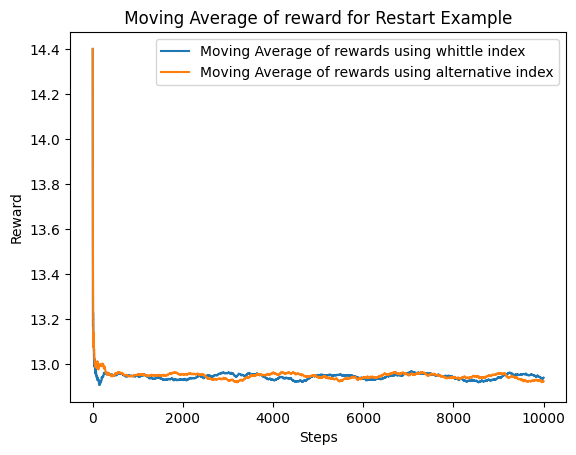
\includegraphics[scale=0.5]{comparison_A_homo_restart.png}
% \caption{Approach A: N=100,M=20}
\begin{center}
\begin{tabular}{cc}
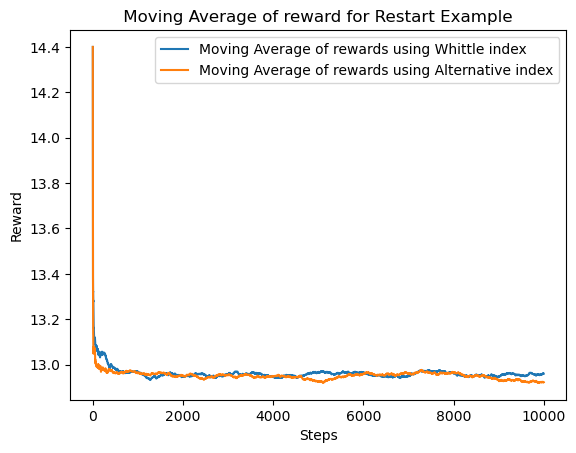
\includegraphics[scale=0.6]{homo_restart_comparison_A.png} &
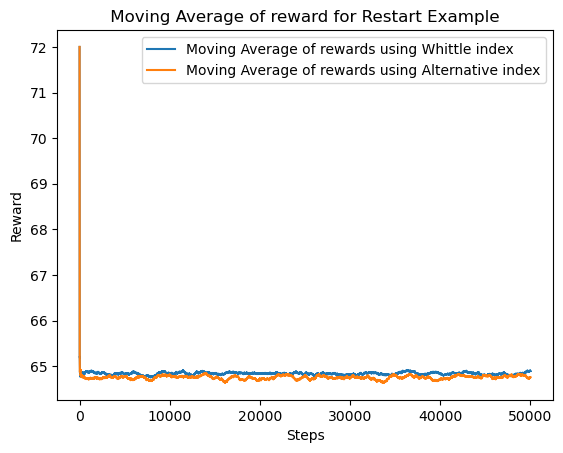
\includegraphics[scale=0.6]{homo_restart_comparison_B.png} \\
\begin{small}
 Approach A: N=20, M=4\end{small} & \begin{small}Approach B, N=100, M=20\end{small}\\
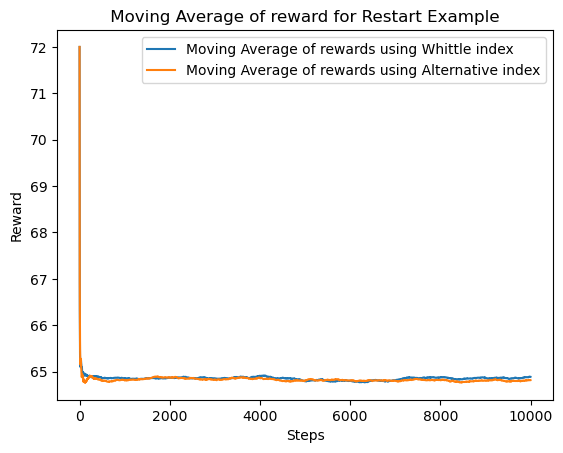
\includegraphics[scale=0.6]{homo_restart_comparison_C.png} &
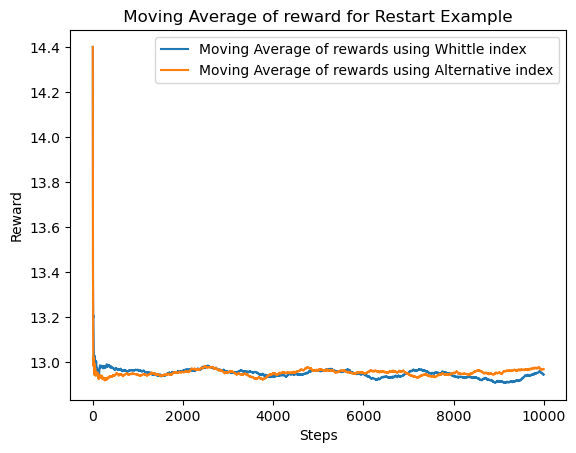
\includegraphics[scale=0.6]{comparison_homo_restart_D_new.png} \\
\begin{small}
 Approach C: N=100, M=20\end{small} & \begin{small}Approach D, N=20, M=4\end{small}\\
 \end{tabular}

\end{center}
    
\newpage
\textbf{Calculating Lagrange indices using DDQN}
\begin{algorithm}[H]
\begin{small}
\begin{algorithmic}[1]
    \State Initialize $\lambda^*$, primary Q network $Q_\theta$, Target Q network $Q_{\theta'}$, Batch Size,$\epsilon$=1.

    % \Function{VisualizationRecommendation}{$B$, $D$, $M$}:
    % \State $\epsilon \gets \text{initialize an error value for terminate condition}$
    % \State $S \gets [S_1, S_2, S_3, ...., S_{
    % |S|}]$  $\text{($|S_{k+1}| > |S_{k}|$ $\forall k \in [1, |S| - 1]$)}$
    % \State $m$ $\gets$ $\text{number of columns of $S_k$}$
    % \State $n$ $\gets$ $\text{number of features per column}$
    \For {n\;=\;1:\;$n_{end}$}
        
        \State Update $\beta(n)$ as:
        $\beta(n)=\frac{1}{\lceil{nlog(n)\backslash5000}\rceil+1}$
        \For{arm $i\in N$}
            \State Choose action $a_{n}^i$ for  arm i in an $\epsilon$-greedy fashion
            \State Update $s_{n+1}^i$ and reward $r_n^i$ from $s_{n}^i$ and $a_{n}^i$ for  arm i
            \State Store $(s_{n}^i,a_{n}^i,r_{n}^i,s_{n+1}^i,\lambda_n^*)$ in experience replay buffer
            \State Train the primary Q network on one batch of $(s_{n},a_{n},r_{n},s_{n+1},\lambda_n^*)$ tuples from experience replay buffer using:
            \Statex\begin{small}
            $Q_{target}(s_n,a_n)\gets(1-a_n)(r_o(s_n)+\lambda_n^*)+a_nr_1(s_n)+\underset{v\epsilon\{0,1\}}{max}Q_{\theta'}(s_{n+1},v)-\frac{1}{2d}\sum\limits_{k\in S}Q_{\theta}(k,0)+Q_{\theta}(k,1)$\end{small}
            % \State Update ($s_n^i$,$a_n^i$) Q-values for each arm i as:
            % \Statex\begin{small}$Q_{n+1}(s_n,a_n)\gets(1-\alpha(n))Q_n(s_n,a_n)+\alpha(n)((1-a_n)(r_o(s_n)+\lambda_n^*)+a_nr_1(s_n)+\underset{v\epsilon\{0,1\}}{max}Q_n(s_{n+1},v)-\frac{1}{2d}\sum\limits_{k\in S}Q_n(k,0)+Q_n(k,1))$\end{small}
        \EndFor
        \State Update the Target Q network 
        \State Update common subsidy for passivity for all arms $\lambda^*$ as: $\lambda_{n+1}^*=\lambda_n^*+\beta(n)(\sum\limits_{i=1}^{i=N}a_n^i-M)$
        
        \State Decrement $\epsilon$ as $\epsilon_{n+1}=max(0.01,\epsilon_{n}*0.99)$
        % \State $total \textunderscore cost \gets 0$
        % \State $\Tilde{y_{k}} \gets$ \text{ranking score of the viz produced using all the features predicted by P}
        % \State $terminate \textunderscore flag \gets False$
        % \While{not $terminate \textunderscore flag$}
        %     \If{$random$ in $[0,1) \leq Pr_{\text {rand}}$} 
        %         \State $ij \gets$ \text{index of a randomly selected unknown feature}
        %     \Else
        %         \State $ij$ $\gets$ $Q(x^{k, t})$ $\text{(index of the feature with the maximum Q value)}$
        %     \EndIf
        %     \State $x^{k, t+1} \gets \text{acquire $f_{ij}$ and unmask it}$
        %     \State $P(x^{k, t}) \gets \text{ranking score predicted using the feature set $x^{k, t}$}$
        %     \State $total \textunderscore cost \gets total \textunderscore cost +\boldsymbol{c}_{\boldsymbol{ij}}$ 
        %     \State $r_{ij}^{k, t} \leftarrow \frac{\left\|\operatorname{P}\left(\boldsymbol{x}^{k,t}\right)-\operatorname{P}\left(\boldsymbol{x}^{k, t+1}\right)\right\|}{\boldsymbol{c}_{ij}} $
        %     \State \text{push} $\left(\boldsymbol{x^{k, t}}, \boldsymbol{x^{k, t+1}}, ij, r_{ij}^{k, t}, \tilde{y_k}\right)$ \text{into the replay memory}
        %     \State $t \leftarrow t+1$
        %     \If{$total \textunderscore cost \geq B$}
        %         \State $terminate \textunderscore flag \gets True$
        %         \State $\hat{y_k} \gets P(x^{k, t})   \text{predicted viz ranking  score on subset of features $x^{k, t}$}$
        %     \EndIf
        %     \State \text{loss} $\gets$ $L(\Tilde{y_k}$,$\hat{y_k})$
        %     \If{$update \textunderscore condition$}
        %         \State \text{train \textunderscore batch} $\gets$ \text{random mini-batch from the replay memory}
        %         \State \text{update Q and target Q networks using train batch }
        %     \EndIf
                
        % \EndWhile
        % \If{$\epsilon > loss$}
        %     terminate loop
        % \EndIf
        
    \EndFor
    \State Calculate the new index for every state s of each arm i by:
        \Statex\hspace*{5mm} $\delta(s)=Q_{\theta}(s,1)-Q_{\theta}(s,0)$
\end{algorithmic}
\end{small}
\end{algorithm}
\newpage
\begin{center}
    
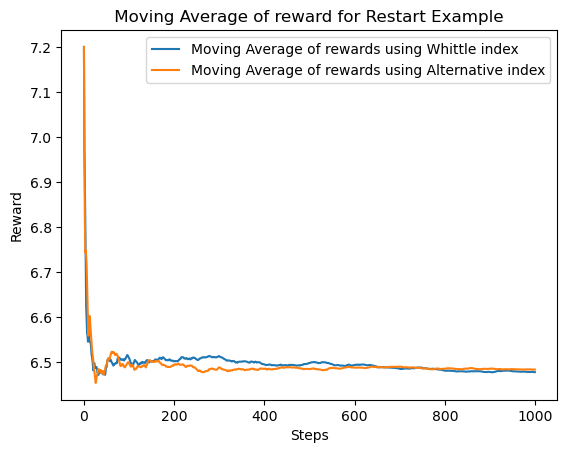
\includegraphics[scale=0.75]{restart_dqn.png}
\end{center}

\begin{center}
    
\begin{small}
\vspace{-10mm}
\hspace{5mm}DDQN: N=10, M=2\end{small}

 \end{center}
\newpage

\textbf{Deadline Scheduling}\\
We study a deadline scheduling problem formulated as RMAB from \textbf{Yu, Z., Xu, Y. and Tong, L., 2018}. This problem, proposed has states formed by two different variables: The service time $B \in$ [0, 9] and
the deadline $T \in$ [0, 12], leading to a total of $|S|$ = 130 states. 

\begin{equation*}
s_{n+1}^i=\begin{cases}
(T_n^i-1, (B_n^i-a_n^i)^+), & \text{if } T_n^i>1 \\
$(T,B)$ \text{ with prob. } $Q(T,B)$, &   \text{if $T_n^i\leq 1$ }

\end{cases}
\end{equation*}
\newpage
If the scheduler reaches the state ($T$ = 1, $B$ $>$ 0), the job could not be finished on time, and an extra penalty
$F(B_n^i-a_n^i)=0.2(B_n^i-a_n^i)^2$ is incurred    
\begin{equation*}
r_{n}^i(s_{n}^i,a_{n}^i,c)=\begin{cases}
(1-c)a_{n}^i, & \text{if } B_n^i>0,T_n^i>1 \\
(1-c)a_{n}^i-F(B_n^i-a_n^i), &   \text{if } B_n^i>0,T_n^i=1\\
0 & \text{otherwise}
\end{cases}
\end{equation*}
\vspace{-1pt}
\noindent The authors provide an expression for Whittle index, given by:
\begin{equation*}
\lambda(T,B,c)=\begin{cases}
0, & \text{if } $B=0$ \\
1-c, &   \text{if } 1\leq B \leq T-1 \\
    
\gamma^{T-1}F(B-T-1)-\\
    \gamma^{T-1}F(B-T)+1-c
& \text{if }
T \leq B
\end{cases}
\end{equation*}
\newpage
In the following results we will consider the homogeneous case using $N$ = 5 and $M$ = 2, with a processing cost c = 0.8. As we are modelling this problem as an average cost MDP we take discount factor $\gamma$=1. We use DDQN approach for this problem as the state space is large
\begin{center}
    
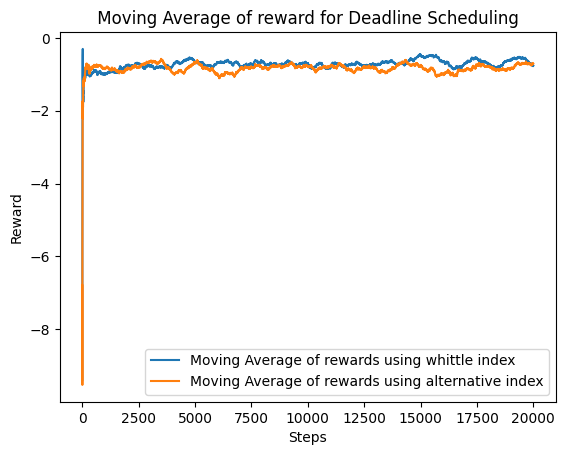
\includegraphics[scale=0.75]{comparison_new.png}
\end{center}
\begin{small}
\vspace{-10mm}
\hspace{100mm}DDQN: N=5, M=2\end{small}
\newpage
\textbf{Non Whittle Indexable Example}\\
The following is a Non-Whittle Indexable problem \textbf{(Gast, N., Gaujal, B. and Khun, K., 2023)} . The transition probability matrices are: 
 \begin{align*}
P_0=
\begin{bmatrix}
0.005 & 0.793 & 0.202\\
0.027 & 558 & 0.415 \\
0.736&0.249&0.015
\end{bmatrix}
\hspace{1mm} \text{and} \hspace{1mm}
P_1=
\begin{bmatrix}
0.718 & 0.254 & 0.028\\
0.347 & 0.097 & 0.556 \\
0.015&0.956&0.029
\end{bmatrix}
\end{align*}
With the Reward Matrix: $[0,0.699],[0,0.362],[0,0.715]$\\
In many Non-Whittle Indexable problems, Whittle indices are used empirically. Hence
even we calculate the Whittle Indices for this problem and compare the performance of our indices against
them.

\newpage
\begin{center}
\begin{tabular}{cc}
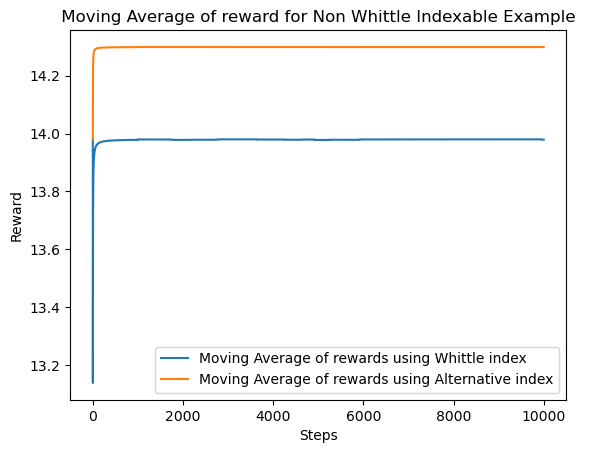
\includegraphics[scale=0.6]{non_whittle_comparison_A.png} &
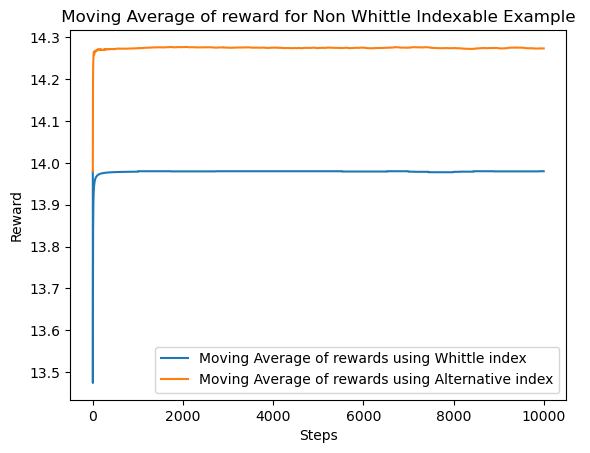
\includegraphics[scale=0.6]{BTP_non_whittle_indexable_B.png} \\
\begin{small}
 Approach A: N=100, M=20\end{small} & \begin{small}Approach B, N=100, M=20\end{small}\\
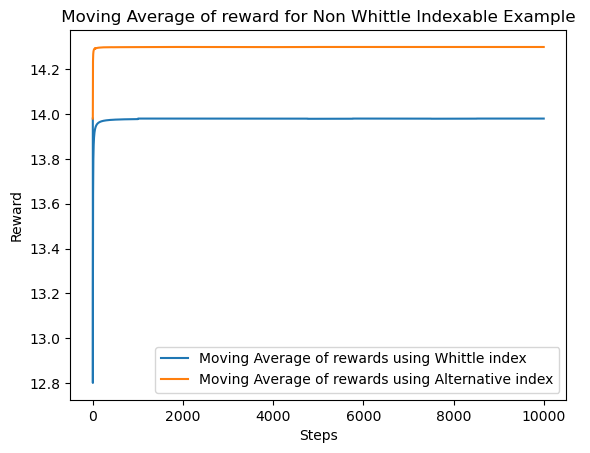
\includegraphics[scale=0.6]{BTP_non_whittle_indexable_C.png} &
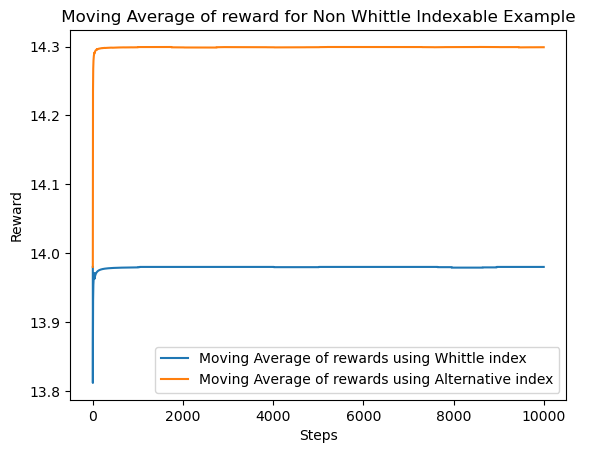
\includegraphics[scale=0.6]{BTP_non_whittle_indexable_D.png} \\
\begin{small}
 Approach C: N=100, M=20\end{small} & \begin{small}Approach D, N=100, M=20\end{small}\\
 \end{tabular}

\end{center}
\newpage
\textbf{Healthcare Workers Problem}\\
This is another problem, from \textbf{Ghosh, A., Nagaraj, D., Jain, M. and Tambe, M., 2022.}, where the Whittle Index Policy is sub-optimal
The example includes two types of arms:
\begin{itemize}
\vspace{-2cm}
    \item Reliable arm:\\
    The Transition Probability Matrices are:\\
    \begin{align*}
    P_0=
    \begin{bmatrix}
    0 & 0 & 1\\
    0 & 0 & 1\\
    0 & 0 & 1
    \end{bmatrix}
    \hspace{1mm} \text{and} \hspace{1mm}
    P_1=
    \begin{bmatrix}
    0& 1 & 0\\
    0 & 1 & 0\\
    0 & 0&1
    \end{bmatrix}
    \end{align*}\\
    The Reward Matrix is: [[0,0],[0.9,0.9],[0,0]]
    \newpage
    \item Greedy arm:\\
    The Transition Probability Matrices are:\\
    \begin{align*}
    P_0=
    \begin{bmatrix}
    0 & 0 & 1\\
    0 & 0 & 1\\
    0 & 0 & 1
    \end{bmatrix}
    \hspace{1mm} \text{and} \hspace{1mm}
    P_1=
    \begin{bmatrix}
    0& 1 & 0\\
    0 & 0 & 1\\
    0 & 0&1
    \end{bmatrix}
    \end{align*}
    The Reward Matrix is: [[0,0],[1.0,1.0],[0,0]]
\end{itemize}
For the experiment we take N=20 (10 reliable arms and 10 greedy arms), M=10 and initialize the reliable arms in the 2nd state and the greedy arms in the 1st state.\\
\newpage
On inspecting the problem we see that the optimal strategy will be to keep activating the Reliable arm when it is in the second state as it remains in this state continuously giving a reward of 0.9. All other cases lead to the arms reaching the recurrent state 3.\\
\begin{center}
    
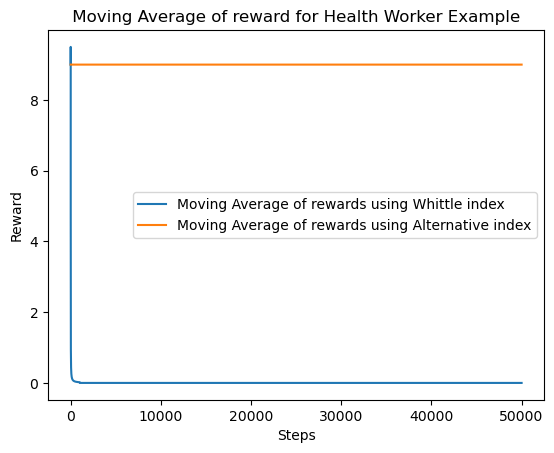
\includegraphics[scale=0.75]{healthcare_worker.png}
\end{center}
\newpage
\vspace{.75in}
\begin{center}
\textit{\textbf{\LARGE \color{red} THANK YOU! }}

\ \\

\textbf{\LARGE \color{144} Best wishes for the next innings, Narahari!}
\end{center}
}



\end{document}